\chapter{Radicaux, carbènes et réarrangements}\label{ch:b3:radicals-carbenes}

Le pyrèthre se défend grâce aux esters de l'acide chrysanthémique, des
molécules construites autour d'un cycle carboné à trois chaînons~; leurs
cousins synthétiques comptent parmi les insecticides domestiques les plus
utilisés. Les chimistes ferment de tels cycles en une étape en additionnant
un \omterm{def:b3:organometallic-bonding:carbene}{carbène} sur une double liaison~: un atome de carbone entouré de six
électrons seulement, dont deux non partagés. Ce chapitre traite
d'intermédiaires réactifs que les volumes de première et de deuxième année
n'ont fait que croiser (radicaux utilisés en synthèse, \omterm{def:b3:organometallic-bonding:carbene}{carbènes} et
\omterm{def:b3:radicals-carbenes:nitrene}{nitrènes}) et des réarrangements dans lesquels un groupe se déplace vers un
atome de carbone, d'azote ou d'oxygène déficitaire en électrons, parmi
lesquels deux qui fabriquent, à partir de la même cétone, les monomères du
nylon-6 et d'un polyester biodégradable.

\begin{recall}
Le volume de première année a introduit les radicaux, l'homolyse et les
flèches à demi-pointe, les carbocations et leurs réarrangements, les
nucléophiles et les groupes partants~; le volume de deuxième année, les
chaînes radicalaires (amorçage, propagation, rupture, amorceurs
radicalaires), les peroxyacides, les lactones, les lactames et les imines.
Le \cref{ch:b3:complex-kinetics} a traité la cinétique des \omterm{def:b3:complex-kinetics:chain}{réactions en
chaîne}, le \cref{ch:b3:organometallic-bonding} les \omterm{def:b3:organometallic-bonding:carbene}{carbènes} comme ligands,
le \cref{ch:b3:many-electron-atoms} les \omterm{def:b3:many-electron-atoms:singlet-triplet}{états singulet} et triplet, et le
\cref{ch:b3:rate-theories} le postulat de Hammond.
\end{recall}

\begin{omfigure}
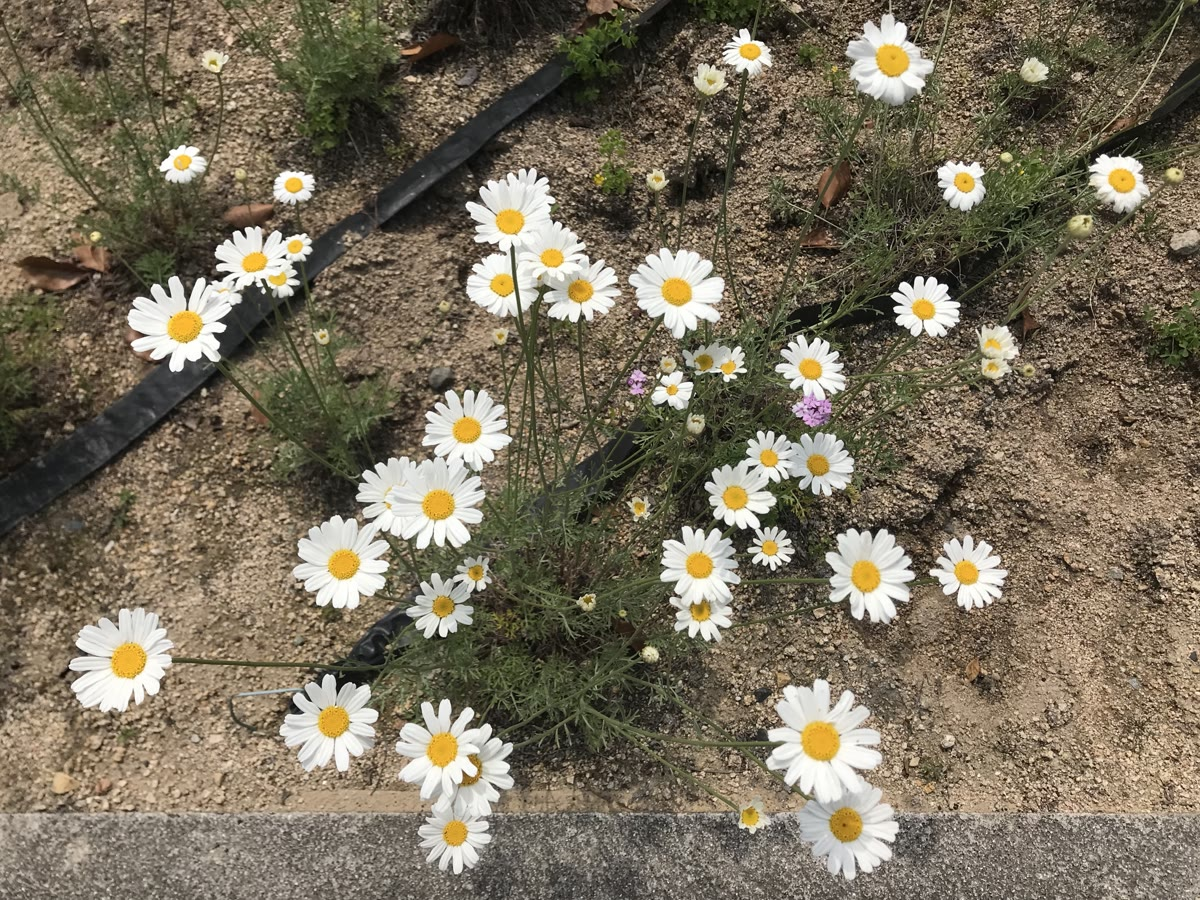
\includegraphics[width=0.48\linewidth]{images/book4/pyrethrum.jpg}

{\small Fleurs de pyrèthre. Elles contiennent les pyréthrines, esters
insecticides d'un acide cyclopropanecarboxylique. Photographie~: Soramimi,
CC BY-SA 4.0.}
\end{omfigure}

\section{Réactions radicalaires en chaîne en synthèse}

La stabilité d'un radical carboné se mesure par l'enthalpie de dissociation
de la liaison C--H qui le formerait~: plus la liaison est faible, plus le
radical est stable.

\begin{proposition}[Enthalpies de dissociation de liaison]\label{prop:b3:radicals-carbenes:bde}
L'enthalpie de dissociation de la liaison R--H à \qty{298}{K} se déduit des enthalpies de formation en phase gazeuse~:
$\mathrm{BDE(R{-}H)} = \Delta_fH^\circ(\mathrm R^\bullet) + \Delta_fH^\circ(\mathrm H^\bullet) - \Delta_fH^\circ(\mathrm{RH})$.
\end{proposition}

\begin{proof}
L'homolyse $\mathrm{RH \to R^\bullet + H^\bullet}$ a, d'après la loi de Hess, pour enthalpie de réaction celle de la formation des produits
moins celle du réactif~; cette enthalpie de réaction est, par définition,
l'enthalpie de dissociation de la liaison.
\end{proof}

\begin{omfigure}
% ledger: dfh4:CH3r, dfh4:C2H5r, dfh4:iC3H7r, dfh4:tC4H9r, dfh4:PhCH2r, dfh4:H, dfh:CH4_g, dfh:C2H6_g, dfh:C3H8_g, dfh4:iC4H10, dfh4:toluene_g
\begin{tikzpicture}
\begin{axis}[width=0.72\linewidth, height=5.2cm, ybar, bar width=16pt, ymin=350, ymax=450,
  xtick={1,2,3,4,5}, xticklabels={{$\ce{CH3-H}$}, {$\ce{C2H5-H}$}, {$\mathrm{(CH_3)_2CH{-}H}$}, {$\mathrm{(CH_3)_3C{-}H}$}, {$\ce{C6H5CH2-H}$}},
  x tick label style={font=\scriptsize}, ylabel={BDE / \unit{kJ.mol^{-1}}},
  axis lines=left, tick label style={font=\scriptsize}, label style={font=\small},
  nodes near coords, nodes near coords style={font=\scriptsize, /pgf/number format/fixed, /pgf/number format/precision=0},
  enlarge x limits=0.15]
\addplot[fill=omDef!55, draw=omDef] table[x=i, y=bde] {figdata/out/bachelor-3-bde.dat};
\end{axis}
\end{tikzpicture}

{\small Enthalpies de dissociation des liaisons C--H à \qty{298}{K},
calculées à partir des enthalpies de formation en phase gazeuse des
molécules et des radicaux~: méthyle, primaire, secondaire, tertiaire et
benzylique. La liaison s'affaiblit à mesure que le radical formé est plus
substitué ou plus conjugué.}
\end{omfigure}

\begin{proposition}[Sélectivité de l'halogénation]\label{prop:b3:radicals-carbenes:halogenation-selectivity}
L'arrachement d'un hydrogène par un atome de brome est bien plus sélectif
entre liaisons C--H primaires, secondaires et tertiaires que l'arrachement
par un atome de chlore.
\end{proposition}

\begin{proof}[Justification]
Comme $\mathrm{BDE(H{-}Cl)}$ dépasse toutes les valeurs C--H de la figure et que $\mathrm{BDE(H{-}Br)}$ leur est inférieure,
l'arrachement par le chlore est exothermique, par le brome endothermique.
D'après le postulat de Hammond (\cref{ch:b3:rate-theories}), l'état de
transition du chlore est précoce, proche des réactifs, et ressent peu la
différence entre les radicaux formés~; celui du brome est tardif, proche
des produits, et son énergie d'activation suit l'essentiel de la
différence de BDE, que le facteur de Boltzmann transforme en grands
rapports de vitesses.
\end{proof}

L'hydrure de tributylétain réduit les halogénures d'alkyle par une chaîne~:
un radical stannylé arrache l'halogène, le radical alkyle arrache un atome
d'hydrogène à la molécule d'hydrure suivante, et un nouveau radical
stannylé se forme. La même chaîne élimine un groupe hydroxy une fois
celui-ci transformé en ester thiocarbonylé (la désoxygénation de
Barton--McCombie), et ferme des cycles. Les résidus organostanniques sont
toxiques et difficiles à éliminer~; le tris(triméthylsilyl)silane et
d'autres silanes remplacent aujourd'hui souvent l'hydrure d'étain.

\begin{omfigure}
\begin{tikzpicture}[font=\small, >=Stealth]
  \node (a) at (-2.0,0) {$\mathrm{Bu_3Sn^\bullet}$};
  \node (b) at (2.0,0) {$\mathrm{R^\bullet}$};
  \draw[->, thick] (a) to[bend left=35] node[midway, above, font=\scriptsize] {$+\,$R--Br, $\ -\,\mathrm{Bu_3SnBr}$} (b);
  \draw[->, thick] (b) to[bend left=35] node[midway, below, font=\scriptsize] {$+\,\mathrm{Bu_3SnH}$, $\ -\,$R--H} (a);
  \node[font=\scriptsize, align=center, anchor=north] at (0,-1.5) {amorçage~: AIBN $\xrightarrow{\Delta}$ 2 R$'^\bullet$ $+$ $\ce{N2}$~; \ R$'^\bullet$ $+$ $\mathrm{Bu_3SnH}$ $\to$ R$'$H $+$ $\mathrm{Bu_3Sn^\bullet}$};
\end{tikzpicture}

{\small Les étapes de propagation de la réduction d'un bromure d'alkyle par
un hydrure d'étain. Chaque R--Br réduit consomme un $\mathrm{Bu_3SnH}$ et donne un $\mathrm{Bu_3SnBr}$~; les \omterm{def:b3:complex-kinetics:chain}{porteurs de chaîne}
sont le radical stannylé et le radical alkyle.}
\end{omfigure}

Le bromure d'hydrogène s'additionne sur les alcènes par le même genre de
chaîne en présence de peroxydes~: un atome de brome s'additionne sur
l'extrémité la moins substituée, ce qui donne le radical le plus stable,
qui arrache ensuite un atome d'hydrogène à HBr~: c'est l'addition
anti-Markovnikov.

\section{Cyclisations radicalaires}

\begin{definition}[Cyclisations exo et endo]\label{def:b3:radicals-carbenes:cyclisation}
Dans une \emph{cyclisation exo}\index{cyclisation exo}, la liaison rompue
(ou la liaison $\pi$ attaquée) se retrouve à l'extérieur du nouveau cycle~; dans une \emph{cyclisation endo}\index{cyclisation endo}, à l'intérieur.
\end{definition}

\begin{omfigure}
\begin{tikzpicture}[font=\scriptsize, >=Stealth]
  % hex-5-enyl radical: C1 radical, C5=C6
  \foreach \i/\a in {1/162, 2/234, 3/306, 4/18} { \coordinate (p\i) at (\a:0.9); }
  \coordinate (p5) at (90:0.95); \coordinate (p6) at (90:1.9);
  \draw[thick] (p1) -- (p2) -- (p3) -- (p4) -- (p5);
  \draw[thick, double, double distance=1.5pt] (p5) -- (p6);
  \node[anchor=east] at (p1) {$\bullet$\,1};
  \node[anchor=west] at (p5) {5}; \node[anchor=west] at (p6) {6};
  \draw[->, omMeth, thick] ($(p1)+(0.1,0.15)$) to[bend left=25] node[pos=0.45, below right, inner sep=1pt] {5-exo} ($(p5)+(-0.15,-0.05)$);
  \draw[->, omThm, thick, densely dashed] ($(p1)+(0,0.25)$) to[bend left=50] node[midway, left] {6-endo} ($(p6)+(-0.2,0)$);
  \node[font=\small, align=center] at (0,-1.6) {radical hex-5-ényle};
  \draw[->, thick] (1.6,0.3) -- (2.7,0.3) node[midway, above] {rapide};
  \begin{scope}[xshift=4.0cm]
    \foreach \i/\a in {1/162, 2/234, 3/306, 4/18, 5/90} { \coordinate (q\i) at (\a:0.75); }
    \draw[thick] (q1) -- (q2) -- (q3) -- (q4) -- (q5) -- (q1);
    \draw[thick] (q5) -- ++(90:0.6) coordinate (q6);
    \node[anchor=south, inner sep=1pt] at (q6) {$\mathrm{{}^\bullet CH_2}$};
    \node[font=\small, align=center] at (0,-1.6) {radical cyclopentylméthyle};
  \end{scope}
\end{tikzpicture}

{\small Le radical hex-5-ényle se ferme par attaque de C1 sur C5 (5-exo, en
vert)~: le nouveau cycle compte cinq chaînons et le radical se retrouve à
l'extérieur, sur C6. L'attaque sur C6 (6-endo, tirets rouges) donnerait le
radical cyclohexyle secondaire, plus stable, mais elle est bien plus
lente~: la chaîne ne peut pas placer C1 sur la ligne d'approche de C6
qu'exige
l'orbitale $\pi^*$.}
\end{omfigure}

\begin{proposition}[Règles de Baldwin]\label{prop:b3:radicals-carbenes:baldwin}
Pour les fermetures de cycle (établies expérimentalement, avec une
justification stéréoélectronique)~: sur un carbone tétraédrique (tet), les
fermetures 3- à 7-exo sont favorisées, 5- et 6-endo défavorisées~; sur un
carbone trigonal (trig), 3- à 7-exo sont favorisées, 3- à 5-endo
défavorisées, 6- et 7-endo favorisées~; sur un carbone digonal (dig), 3- et
4-exo sont défavorisées, 5- à 7-exo favorisées, 3- à 7-endo favorisées.
\end{proposition}

La justification tient à l'angle d'attaque qu'exige chaque type de
liaison~: par l'arrière de la liaison sur un carbone tet, à environ 107° sur
un système $\pi$ trigonal, sous un angle plus fermé sur une triple liaison~; une
chaîne courte ne peut pas atteindre ces positions dans les cas
défavorisés.

\begin{definition}[Horloge radicalaire]\label{def:b3:radicals-carbenes:radical-clock}
Une \emph{horloge radicalaire}\index{horloge radicalaire} est un radical
qui se réarrange de façon unimoléculaire avec une constante de vitesse
connue, comme le radical hex-5-ényle qui se cyclise~; sa compétition avec un
piège bimoléculaire mesure la constante de vitesse du piège, ou
l'inverse.
\end{definition}

\begin{proposition}[Cinétique de compétition]\label{prop:b3:radicals-carbenes:clock}
Si un radical soit se cyclise ($k_c$), soit est piégé par un hydrure maintenu en excès à la
concentration $[\mathrm{R_3SnH}]$ ($k_H$), le rapport des produits vaut
$[\text{cyclisé}]/[\text{direct}] = k_c/(k_H[\mathrm{R_3SnH}])$.
\end{proposition}

\begin{proof}
À chaque instant, les deux produits se forment respectivement avec les vitesses $k_c[\mathrm R^\bullet]$ et $k_H[\mathrm{R_3SnH}][\mathrm R^\bullet]$. Leur rapport
ne dépend pas de la concentration du radical, qui varie~; la concentration
en hydrure étant constante, l'intégration sur le temps multiplie les deux par le même
$\int[\mathrm R^\bullet]\,\dd t$, et le rapport des produits est le rapport des constantes de vitesse
multiplié par $1/[\mathrm{R_3SnH}]$.
\end{proof}

\begin{omfigure}
\begin{tikzpicture}
\begin{axis}[name=a, width=0.47\linewidth, height=5.2cm, xmode=log, xmin=1e-3, xmax=1, ymin=0, ymax=1,
  axis lines=left, xlabel={$[\mathrm{Bu_3SnH}]$ / \unit{mol.L^{-1}}}, ylabel={fraction cyclisée},
  tick label style={font=\scriptsize}, label style={font=\small}]
\addplot[omDef, thick] table[x=c, y=fcyc] {figdata/out/bachelor-3-radical-clock.dat};
\end{axis}
\begin{axis}[at={(a.east)}, anchor=west, xshift=1.5cm, width=0.47\linewidth, height=5.2cm,
  xmin=0, xmax=1, ymin=0, ymax=11, axis lines=left,
  xlabel={$[\mathrm{Bu_3SnH}]$ / \unit{mol.L^{-1}}}, ylabel={[direct]/[cyclisé]},
  tick label style={font=\scriptsize}, label style={font=\small}]
\addplot[omThm, thick] table[x=c, y=inv] {figdata/out/bachelor-3-radical-clock-b.dat};
\node[font=\scriptsize, anchor=west, omThm] at (axis cs:0.15,7.5) {pente $k_H/k_c$};
\end{axis}
\end{tikzpicture}

{\small L'horloge hex-5-ényle avec les constantes de vitesse du modèle $k_c = \qty{2.3e5}{s^{-1}}$ et
$k_H = \qty{2.4e6}{L.mol^{-1}.s^{-1}}$. À gauche~: fraction de méthylcyclopentane parmi les produits en fonction de la
concentration en hydrure~: la moitié pour $k_c/k_H \approx \qty{0.1}{mol/L}$. À droite~: le rapport inverse est une droite
passant par l'origine, de pente $k_H/k_c$.}
\end{omfigure}

\begin{method}[Concevoir une réduction ou une cyclisation radicalaire]\label{met:b3:radicals-carbenes:radical-chain}
\begin{enumerate}
  \item Pour une simple réduction, maintenir le donneur d'hydrogène
        concentré (environ \qty{0.1}{mol/L} ou plus) afin que le radical soit piégé avant de se réarranger.
  \item Pour une cyclisation, maintenir le donneur dilué, ou l'ajouter
        lentement, afin que le radical se cyclise d'abord~: choisir $[\text{donneur}] \ll k_c/k_H$.
  \item Choisir un amorceur dont la demi-vie à la température de réaction
        est de l'ordre de la durée de la réaction (AIBN vers \qty{80}{\celsius}), et l'ajouter par portions si
        nécessaire.
  \item Préférer un silane ou un autre donneur sans étain, et éliminer le
        dioxygène, qui piège les radicaux carbonés.
\end{enumerate}
\end{method}

\begin{inthelab}[Addition lente au pousse-seringue]
Pour maintenir un réactif dilué pendant toute une réaction, on charge sa
solution dans une seringue étanche aux gaz et on l'ajoute à travers un
septum au moyen d'un pousse-seringue pendant plusieurs heures, dans la
solution du substrat à reflux sous diazote. La concentration du réactif
reste alors voisine de sa faible valeur stationnaire, fixée par la vitesse
d'addition et la vitesse à laquelle il est consommé.
\end{inthelab}

\section{Carbènes}

\begin{definition}[Carbènes singulet et triplet]\label{def:b3:radicals-carbenes:carbene-states}
Un \emph{carbène singulet}\index{carbene singulet@carbène singulet} a ses deux électrons non
liants appariés dans une même orbitale, un hybride $sp^2$, son orbitale p étant vide~; un
\emph{carbène triplet}\index{carbene triplet@carbène triplet} les a non appariés, un dans
chaque orbitale, avec des spins parallèles.
\end{definition}

\begin{omfigure}
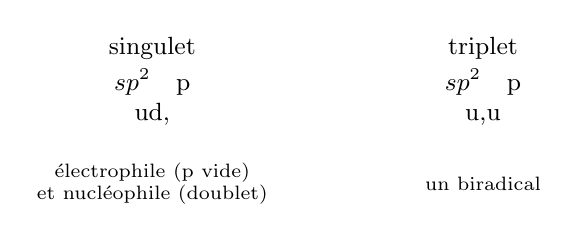
\begin{tikzpicture}[font=\small]
  \node[align=center] at (0,0) {singulet\\[2pt] $sp^2$ \ \ p\\ \omorbs{ud,}};
  \node[align=center] at (4.2,0) {triplet\\[2pt] $sp^2$ \ \ p\\ \omorbs{u,u}};
  \node[font=\scriptsize, align=center] at (0,-1.3) {électrophile (p vide)\\ et nucléophile (doublet)};
  \node[font=\scriptsize, align=center] at (4.2,-1.3) {un biradical};
\end{tikzpicture}

{\small Occupation électronique des deux orbitales non liantes d'un \omterm{def:b3:organometallic-bonding:carbene}{carbène}.
Le triplet est l'état fondamental de $\ce{CH2}$~; des substituants $\pi$-donneurs (Cl, OR, $\mathrm{NR_2}$) élèvent l'orbitale
p et font du singulet l'état fondamental, comme dans le dichlorocarbène.}
\end{omfigure}

Les \omterm{def:b3:organometallic-bonding:carbene}{carbènes} se préparent par perte de diazote à partir d'un composé diazo
(par chauffage, irradiation ou catalyse métallique), par $\alpha$-élimination (le chloroforme et une base forte donnent
$\ce{CCl3-}$, qui perd un chlorure pour donner $\ce{CCl2}$), ou sont évités tout à fait grâce à un
\omterm{def:b3:radicals-carbenes:carbenoid}{carbénoïde}.

\begin{definition}[Carbénoïdes]\label{def:b3:radicals-carbenes:carbenoid}
Un \emph{carbénoïde}\index{carbenoide@carbénoïde} est une espèce liée à un métal qui transfère
un groupe \omterm{def:b3:organometallic-bonding:carbene}{carbène} comme le ferait un \omterm{def:b3:organometallic-bonding:carbene}{carbène} libre, sans que celui-ci se
forme, comme l'iodure d'iodométhylzinc $\ce{ICH2ZnI}$ de la réaction de Simmons--Smith.
\end{definition}

\begin{definition}[Cyclopropanation]\label{def:b3:radicals-carbenes:cyclopropanation}
La \emph{cyclopropanation}\index{cyclopropanation} est la formation d'un
cyclopropane par addition d'un \omterm{def:b3:organometallic-bonding:carbene}{carbène} ou d'un \omterm{def:b3:radicals-carbenes:carbenoid}{carbénoïde} sur une double
liaison C=C.
\end{definition}

\begin{proposition}[Le test de Skell]\label{prop:b3:radicals-carbenes:skell}
Un \omterm{def:b3:radicals-carbenes:carbene-states}{carbène singulet} s'additionne sur un alcène \textit{cis} ou \textit{trans} de façon
stéréospécifique, en conservant la configuration relative~; un \omterm{def:b3:radicals-carbenes:carbene-states}{carbène
triplet} donne les deux stéréoisomères du cyclopropane.
\end{proposition}

\begin{proof}[Justification]
Le singulet forme les deux nouvelles liaisons en une seule étape concertée,
sans laisser le temps à une rotation. Le triplet forme d'abord une liaison,
ce qui donne un biradical-1,3 triplet~; ses deux électrons non appariés ne
peuvent former la seconde liaison qu'après le retournement d'un spin,
lent par rapport à la rotation autour de la liaison simple C--C restante~:
la configuration est brouillée.
\end{proof}

\begin{omfigure}
\setchemfig{atom sep=1.8em}
\schemestart
\chemfig{H_3C-[:30]=[:0]-[:-30]CH_3}
\arrow{->[$\ce{CH2}$ singulet]}[,1.6]
\chemfig{(<[:210]H_3C)-[:0](<[:330]CH_3)-[:120]-[:240]}
\schemestop
\par\medskip

{\small Le test de Skell~: le \textit{cis}-but-2-ène, aux deux groupes méthyle du même côté, ne donne avec
un \omterm{def:b3:radicals-carbenes:carbene-states}{carbène singulet} que le \textit{cis}-1,2-diméthylcyclopropane (les deux groupes méthyle en coins pleins,
sur la même face du cycle)~; avec un \omterm{def:b3:radicals-carbenes:carbene-states}{carbène
triplet}, l'isomère \textit{trans} apparaît aussi.}
\end{omfigure}

Les \omterm{def:b3:radicals-carbenes:carbene-states}{carbènes singulets} s'insèrent aussi dans les liaisons C--H. Les
carboxylates de rhodium(II) décomposent les diazoesters en \omterm{def:b3:radicals-carbenes:carbenoid}{carbénoïdes} du
rhodium qui cyclopropanent les alcènes et s'insèrent sélectivement dans les
liaisons C--H, et, avec des ligands chiraux, de façon énantiosélective.

\begin{definition}[Nitrènes]\label{def:b3:radicals-carbenes:nitrene}
Un \emph{nitrène}\index{nitrene@nitrène} $\mathrm{R{-}\ddot N}$ est l'analogue azoté d'un \omterm{def:b3:organometallic-bonding:carbene}{carbène}, un atome
d'azote neutre entouré de six électrons seulement, formé par exemple par
perte de diazote à partir d'un azoture.
\end{definition}

\section{Réarrangements vers un carbone déficitaire en électrons}

\begin{definition}[Migration 1,2]\label{def:b3:radicals-carbenes:shift}
Une \emph{migration 1,2}\index{migration 1,2} est le déplacement d'un
groupe, avec son doublet liant, d'un atome vers l'atome voisin déficitaire
en électrons.
\end{definition}

Dans une migration de Wagner--Meerwein, un groupe alkyle ou un hydrure se
déplace vers un carbocation voisin, ce qui en donne un plus stable~: ce sont
les réarrangements de carbocations du volume de première année, dont le
mécanisme reçoit maintenant un nom. Dans la nature, les squelettes
terpéniques sont remodelés par des cascades de telles migrations.

\begin{definition}[Réarrangement pinacolique]\label{def:b3:radicals-carbenes:pinacol}
Le \emph{réarrangement pinacolique}\index{rearrangement pinacolique@réarrangement pinacolique} transforme un
diol-1,2, en milieu acide, en une cétone ou un aldéhyde~: un groupe hydroxy
part sous forme d'eau, un groupe porté par le carbone voisin migre vers le
cation, et le cation formé, stabilisé par l'oxygène restant, perd un
proton.
\end{definition}

\begin{definition}[Aptitude migratoire]\label{def:b3:radicals-carbenes:migratory}
L'\emph{aptitude migratoire}\index{aptitude migratoire} d'un groupe est sa
tendance relative à se déplacer, lors d'une \omterm{def:b3:radicals-carbenes:shift}{migration 1,2}, vers un centre
déficitaire en électrons.
\end{definition}

Les groupes qui portent bien une charge positive pendant la migration
migrent le mieux~: l'hydrure, les aryles et les alkyles tertiaires avant
les secondaires, les primaires et le méthyle. Le pinacol,
$\mathrm{(CH_3)_2C(OH){-}C(OH)(CH_3)_2}$, donne la pinacolone, la 3,3-diméthylbutan-2-one.

\begin{method}[Prévoir le produit d'un réarrangement]\label{met:b3:radicals-carbenes:rearrangement}
\begin{enumerate}
  \item Trouver l'atome déficitaire en électrons qui se forme (cation,
        nitrénium, oxygène d'un peroxyde activé, \omterm{def:b3:organometallic-bonding:carbene}{carbène} ou \omterm{def:b3:radicals-carbenes:nitrene}{nitrène}) et le
        groupe partant qui le crée.
  \item Lister les groupes de l'atome voisin susceptibles de migrer~;
        lorsque la géométrie est figée (oximes), seul le groupe anti par
        rapport au groupe partant le peut.
  \item Sinon, choisir selon l'\omterm{def:b3:radicals-carbenes:migratory}{aptitude migratoire}, ou selon le groupe qui
        forme le cation le plus stable à l'endroit qu'il quitte.
  \item Déplacer le groupe avec rétention de sa configuration, puis
        compléter le mécanisme (perte d'un proton, addition d'eau).
\end{enumerate}
\end{method}

\section{Réarrangements vers un azote ou un oxygène déficitaire en électrons}

\begin{definition}[Réarrangement de Beckmann]\label{def:b3:radicals-carbenes:beckmann}
Le \emph{réarrangement de Beckmann}\index{rearrangement de Beckmann@réarrangement de Beckmann} transforme une
oxime, en milieu acide fort, en un amide~: le groupe hydroxy, activé en
groupe partant, s'en va tandis que le groupe situé en anti migre du carbone
vers l'azote~; l'eau s'additionne sur l'ion nitrilium formé, et une
tautomérie donne l'amide.
\end{definition}

\begin{proposition}[Migration anti]\label{prop:b3:radicals-carbenes:beckmann-anti}
Dans le \omterm{def:b3:radicals-carbenes:beckmann}{réarrangement de Beckmann}, le groupe qui migre est celui qui est
en anti par rapport au groupe partant porté par l'azote.
\end{proposition}

\begin{proof}[Justification]
Le doublet de la liaison qui migre attaque l'azote par l'arrière de la
liaison N--O, comme dans une substitution
$\mathrm S_\mathrm N2$~; seul le groupe en anti par rapport à l'oxygène a sa liaison alignée avec
l'orbitale $\sigma^*$ N--O. L'étape est concertée avec le départ du groupe partant,
si bien qu'il ne se forme aucun ion nitrénium libre qui pourrait choisir
autrement.
\end{proof}

\begin{omfigure}
\setchemfig{atom sep=1.9em}
\schemestart
\chemfig{*6(-----(=N-[:30]OH)-)}
\arrow{->[$\ce{H2SO4}$ (oleum)][Beckmann]}[,1.8]
\chemfig{*7(---N(-[:-90]H)-(=O)---)}
\schemestop
\par\medskip
\schemestart
\chemfig{*6(-----(=O)-)}
\arrow{->[peroxyacide][Baeyer--Villiger]}[,1.8]
\chemfig{*7(-----O-(=O)-)}
\schemestop

{\small Deux agrandissements de cycle de la cyclohexanone. En haut~: son
oxime se réarrange dans l'oléum en caprolactame (azépan-2-one), le monomère
du nylon-6, l'azote entrant dans le cycle. En bas~: un peroxyacide insère
un atome d'oxygène à côté du groupe carbonyle, ce qui donne la
$\varepsilon$-caprolactone (oxépan-2-one).}
\end{omfigure}

\begin{definition}[Oxydation de Baeyer--Villiger]\label{def:b3:radicals-carbenes:baeyer}
L'\emph{oxydation de Baeyer--Villiger}\index{oxydation de Baeyer--Villiger} transforme une
cétone en ester, ou une cétone cyclique en lactone, par un peroxyacide~: le
peroxyacide s'additionne sur le groupe carbonyle, puis un groupe porté par
le carbone du carbonyle migre vers l'oxygène peroxydique le plus proche
tandis qu'un carboxylate s'en va.
\end{definition}

\begin{proposition}[Régiochimie de Baeyer--Villiger]\label{prop:b3:radicals-carbenes:bv-retention}
Dans l'\omterm{def:b3:radicals-carbenes:baeyer}{oxydation de Baeyer--Villiger}, le groupe qui migre conserve sa
configuration, et l'ordre des \omterm{def:b3:radicals-carbenes:migratory}{aptitudes migratoires} est alkyle tertiaire >
alkyle secondaire $\approx$ aryle > alkyle primaire > méthyle (établi expérimentalement).
\end{proposition}

\begin{proof}[Justification]
Le groupe se déplace avec son doublet liant le long de la face du carbone
qu'il quitte et atterrit sur l'oxygène du même côté, si bien que sa
configuration est conservée. Dans l'état de transition, le groupe qui
migre porte une charge positive partielle, que la substitution alkyle et
la conjugaison aryle stabilisent.
\end{proof}

\begin{definition}[Isocyanates, réarrangements de Curtius et de Hofmann]\label{def:b3:radicals-carbenes:curtius}
Un \emph{isocyanate}\index{isocyanate} est un composé $\ce{R-N=C=O}$. Dans le \emph{réarrangement de Curtius}\index{rearrangement de Curtius@réarrangement de Curtius}, un azoture d'acyle perd du diazote par
chauffage tandis que le groupe R migre du carbone vers l'azote, ce qui donne
un isocyanate~; dans le \emph{réarrangement de Hofmann}\index{rearrangement de Hofmann@réarrangement de Hofmann}, un amide
primaire traité par le dibrome et une base donne le même isocyanate en
passant par un N-bromoamide. Avec l'eau, l'isocyanate donne l'amine $\ce{RNH2}$ et du dioxyde
de carbone~; avec un alcool, un carbamate.
\end{definition}

\begin{definition}[Cétènes et réarrangement de Wolff]\label{def:b3:radicals-carbenes:wolff}
Un \emph{cétène}\index{cetene@cétène} est un composé $\mathrm{R_2C{=}C{=}O}$. Dans le \emph{réarrangement de Wolff}\index{rearrangement de Wolff@réarrangement de Wolff}, une $\alpha$-diazocétone perd du diazote
tandis que le groupe porté par le carbone du carbonyle migre, ce qui donne
un cétène, qui additionne l'eau, un alcool ou une amine.
\end{definition}

Le \omterm{def:b3:radicals-carbenes:wolff}{réarrangement de Wolff} est l'étape clé de l'homologation
d'Arndt--Eistert, qui allonge un acide carboxylique d'un carbone~: chlorure
d'acide, puis diazocétone, puis \omterm{def:b3:radicals-carbenes:wolff}{cétène}, puis l'acide homologue.

\begin{safety}{\ghs[0.62cm]{GHS06}\ghs[0.62cm]{GHS08}\ghs[0.62cm]{GHS09}}
% ledger: ghs4:Bu3SnH, ghs4:diazomethane, ghs4:AIBN
Hydrure de tributylétain~: toxique en cas d'ingestion, nocif par contact
cutané, risque avéré d'effets graves pour les organes à la suite
d'expositions répétées, très toxique pour les organismes aquatiques~; les
résidus d'étain sont collectés séparément. Le diazométhane est un gaz
toxique, cancérogène et explosif~; il n'est cité ici que pour sa chimie et
on le remplace en pratique par des réactifs plus sûrs comme le
triméthylsilyldiazométhane. L'AIBN est autoréactif à la chaleur.
\end{safety}

\begin{history}[Un radical qui ne devait pas exister, et un nylon]
En 1900, Moses Gomberg, qui cherchait à préparer l'hexaphényléthane,
obtint une solution jaune qui fixait le dioxygène et le diiode~: le radical
triphénylméthyle, premier radical carboné persistant. Un demi-siècle plus
tard, le \omterm{def:b3:radicals-carbenes:beckmann}{réarrangement de Beckmann} de l'oxime de la cyclohexanone devint la
voie industrielle vers le caprolactame, polymérisé par ouverture de cycle en
nylon-6, une fibre et une matière plastique technique produites à très
grande échelle.
\end{history}

\section{Exercices}

\begin{exercise}[$\star$]\label{exo:b3:radicals-carbenes:1}
À \qty{25}{\celsius}, les réactivités relatives par hydrogène des liaisons C--H primaires, secondaires et
tertiaires valent $1 : 3.9 : 5.1$ vis-à-vis des atomes de chlore et $1 : 82 : 1600$ vis-à-vis des
atomes de brome (données de l'exercice). Calculer les proportions de 1- et
de 2-halogénopropane formées à partir du propane dans chaque cas.
\end{exercise}

\begin{exercise}[$\star$]\label{exo:b3:radicals-carbenes:2}
Quel est l'état fondamental de $\ce{CH2}$, et de $\ce{CCl2}$~? Lequel s'additionne de façon stéréospécifique sur le
\textit{trans}-but-2-ène, et que donne-t-il~?
\end{exercise}

\begin{exercise}[$\star$]\label{exo:b3:radicals-carbenes:3}
Donner le produit de la réaction de Simmons--Smith du (\textit{Z})-hex-3-ène.
\end{exercise}

\begin{exercise}[$\star$]\label{exo:b3:radicals-carbenes:4}
Donner les produits de l'\omterm{def:b3:radicals-carbenes:baeyer}{oxydation de Baeyer--Villiger} de la cyclohexanone
et de l'acétophénone.
\end{exercise}

\begin{exercise}[$\star\star$]\label{exo:b3:radicals-carbenes:5}
Avec les données de l'\cref{exo:b3:radicals-carbenes:1}, calculer les
proportions des deux monochlorures et des deux monobromures du
2-méthylpropane.
\end{exercise}

\begin{exercise}[$\star\star$]\label{exo:b3:radicals-carbenes:6}
Une nouvelle \omterm{def:b3:radicals-carbenes:radical-clock}{horloge radicalaire}, réduite par $\qty{0.020}{mol/L}$ de $\mathrm{Bu_3SnH}$, donne trois fois plus de produit réarrangé
que de produit non réarrangé. Avec $k_H = \qty{2.4e6}{L.mol^{-1}.s^{-1}}$, trouver sa constante de vitesse.
\end{exercise}

\begin{exercise}[$\star\star$]\label{exo:b3:radicals-carbenes:7}
Classer selon les règles de Baldwin l'attaque d'un radical hex-5-ényle sur
C5 et sur C6, puis dire si chacune des fermetures suivantes est
favorisée~: 4-exo-tet, 5-endo-trig, 5-exo-dig, 3-exo-dig, 5-endo-dig.
\end{exercise}

\begin{exercise}[$\star\star$]\label{exo:b3:radicals-carbenes:8}
Donner le produit du \omterm{def:b3:radicals-carbenes:pinacol}{réarrangement pinacolique} du
2,3-diphénylbutane-2,3-diol, et expliquer le choix du groupe qui migre.
\end{exercise}

\begin{exercise}[$\star\star$]\label{exo:b3:radicals-carbenes:9}
L'azoture de benzoyle est chauffé dans le toluène, puis on ajoute de
l'eau~; dans une seconde expérience, de l'éthanol. Donner les produits.
\end{exercise}

\begin{exercise}[$\star\star\star$]\label{exo:b3:radicals-carbenes:10}
Avec $\mathrm{BDE(H{-}Cl)} = \qty{432}{kJ/mol}$ et $\mathrm{BDE(H{-}Br)} = \qty{366}{kJ/mol}$ (données de l'exercice) et les valeurs C--H de
la figure du chapitre, calculer $\Delta H$ pour l'arrachement d'un hydrogène primaire et d'un hydrogène tertiaire
par chaque atome d'halogène, et utiliser le postulat de Hammond pour
expliquer les sélectivités de l'\cref{exo:b3:radicals-carbenes:1}.
\end{exercise}

\begin{exercise}[$\star\star\star$]\label{exo:b3:radicals-carbenes:11}
Donner les produits de Beckmann des deux oximes, \textit{E} et \textit{Z}, de la 2-méthylcyclohexanone,
et expliquer pourquoi ils diffèrent, alors que l'\omterm{def:b3:radicals-carbenes:baeyer}{oxydation de
Baeyer--Villiger} de la cétone donne une lactone principale.
\end{exercise}

\begin{exercise}[$\star\star\star$]\label{exo:b3:radicals-carbenes:12}
Avec l'horloge modèle du chapitre, calculer la fraction cyclisée pour $[\mathrm{Bu_3SnH}] = 0.010$,
0.10 et \qty{1.0}{mol/L}. Quelle concentration en hydrure donne 95\,\% de produit cyclisé, et comment
peut-on la maintenir~?
\end{exercise}

\section{Problème~: deux cycles à partir de la cyclohexanone}

\begin{problem}[{Problème du week-end --- deux cycles à partir de la
cyclohexanone~: l'oxime, le réarrangement de Beckmann en caprolactame,
l'oxydation de Baeyer--Villiger en caprolactone, et la régiochimie des deux
avec la 2-méthylcyclohexanone}]
\label{pb:b3:radicals-carbenes:1}
% ledger: aw:C, aw:H, aw:N, aw:O, aw:S
Données du problème~: une tonne de cyclohexanone est convertie en son oxime
avec un rendement de 98\,\%, et l'oxime en caprolactame avec un rendement
de 98\,\%~; le réarrangement consomme 1.3 mol d'acide sulfurique (sous forme
d'oléum) par mole d'oxime, neutralisé à la fin par l'ammoniac en sulfate
d'ammonium.

\medskip\noindent\textbf{Partie I --- L'oxime.}
\begin{enumerate}
  \item Écrire la formation de l'oxime de la cyclohexanone à partir de
        l'hydroxylamine.
  \item Pourquoi opère-t-on vers pH 4 à 5~?
  \item L'oxime de la cyclohexanone a-t-elle des isomères \textit{E} et \textit{Z}~? Pourquoi~?
  \item Dessiner les oximes \textit{E} et \textit{Z} de la 2-méthylcyclohexanone.
  \item Pourquoi ces deux oximes ne s'interconvertissent-elles que
        lentement~?
\end{enumerate}

\medskip\noindent\textbf{Partie II --- Le \omterm{def:b3:radicals-carbenes:beckmann}{réarrangement de Beckmann}.}
\begin{enumerate}[resume]
  \item Que fait l'acide à l'oxime~?
  \item Quelle liaison migre, et pourquoi le cycle s'agrandit-il~?
  \item Quel intermédiaire l'eau attaque-t-elle~?
  \item Écrire l'équation globale, de l'oxime au caprolactame.
  \item Nommer et dessiner le produit, ainsi que le polymère qui en est
        issu.
  \item Calculer les masses molaires de la cyclohexanone et du caprolactame.
  \item Calculer la masse de caprolactame obtenue à partir d'une tonne de
        cyclohexanone.
  \item Calculer la masse de sulfate d'ammonium formée en même temps.
\end{enumerate}

\medskip\noindent\textbf{Partie III --- L'\omterm{def:b3:radicals-carbenes:baeyer}{oxydation de Baeyer--Villiger}.}
\begin{enumerate}[resume]
  \item Écrire l'oxydation de la cyclohexanone par un peroxyacide $\ce{RCO3H}$.
  \item Donner l'intermédiaire formé par addition du peroxyacide.
  \item Quel groupe migre, et quel est le groupe partant~?
  \item Nommer la lactone et le polymère qu'elle donne.
  \item Pourquoi le peroxyde d'hydrogène associé à un catalyseur peut-il
        remplacer le peroxyacide dans un procédé plus propre~?
\end{enumerate}

\medskip\noindent\textbf{Partie IV --- La 2-méthylcyclohexanone.}
\begin{enumerate}[resume]
  \item Quel carbone migre lors de son \omterm{def:b3:radicals-carbenes:baeyer}{oxydation de Baeyer--Villiger}, et
        quelle lactone se forme~?
  \item La configuration de ce carbone est-elle conservée~?
  \item Quel lactame l'oxime \textit{E} donne-t-elle (OH en anti par rapport au carbone porteur du méthyle)~?
  \item Quel lactame l'oxime \textit{Z} donne-t-elle~?
  \item Qu'est-ce qui décide de la régiochimie dans chaque réaction~?
  \item Pourquoi la cyclohexanone elle-même échappe-t-elle à ces
        problèmes~?
  \item Énoncer le résultat~: la masse de caprolactame obtenue à partir
        d'une tonne de cyclohexanone.
\end{enumerate}
\end{problem}
